\documentclass[journal]{IEEEtran}

% *** GRAPHICS RELATED PACKAGES ***
%
\ifCLASSINFOpdf
  \usepackage[pdftex]{graphicx}
  % declare the path(s) where your graphic files are
  \graphicspath{{../images/}}
  % and their extensions so you won\'t have to specify these with
  % every instance of \includegraphics
  \DeclareGraphicsExtensions{.pdf,.jpeg,.png}
\else
  % or other class options (dvipsone, dvipdfx, etc.) graphicx for EPS,
  % graphicx for PDF, graphics for both
  \usepackage[dvips]{graphicx}
  % declare the path(s) where your graphic files are
  \graphicspath{{../eps/}}
  % and their extensions so you won\'t have to specify these with
  % every instance of \includegraphics
  \DeclareGraphicsExtensions{.eps}
\fi

\usepackage{amsmath}
\usepackage{amsfonts}
\usepackage{amssymb}
\usepackage{algpseudocode}
\usepackage{array}
\usepackage{booktabs}
\usepackage{multirow}
\usepackage{lipsum}
\usepackage{hyperref}


% correct bad hyphenation here
\hyphenation{op-tical net-works semi-con-duc-tor}


\begin{document}

\title{Synthesizing Agile, SSDLC and AIOps}

\author{
    \IEEEauthorblockN{Mathew Raio III,}
    \IEEEauthorblockA{Independent Researcher, Snohomish County, WA\\
    Email: mathew.raio@csuglobal.edu}
    \and
    \IEEEauthorblockN{Gemini AI,}
    \IEEEauthorblockA{Compiler and Co-author}
}

\maketitle

\begin{abstract}
This paper presents a novel framework that integrates Agile methodologies, the Secure Software Development Lifecycle (SSDLC), and Artificial Intelligence for IT Operations (AIOps). The proposed framework addresses the growing complexity of software development by creating a cohesive workflow that is acceptable to both business and research facilities. By embedding security and AI-driven automation into the core of the Agile process, this framework aims to enhance feedback loops, accelerate delivery, and improve the overall quality and security of software systems.
\end{abstract}

\begin{IEEEkeywords}
AIOps, Agile, SDLC, SSDLC, DevOps, Software Engineering, Automation, Machine Learning, Context Engineering.
\end{IEEEkeywords}

\section{Introduction}
The modern software development landscape is defined by a need for speed, security, and reliability. Agile methodologies have enabled rapid, iterative development, but the increasing complexity of software systems and the constant threat of security vulnerabilities require a more integrated approach. The Secure Software Development Lifecycle (SSDLC) provides a model for building security into every phase of development, while AIOps offers the potential to automate and optimize IT operations through artificial intelligence.

This paper proposes a unified framework that synthesizes these three powerful paradigms: Agile, SSDLC, and AIOps. We argue that by weaving security and AI-driven insights into the fabric of the Agile process, organizations can create a more resilient, efficient, and secure software development lifecycle. This integrated approach, which we call the "Secure AIOps-driven Agile Framework," is designed to be adaptable for both fast-paced business environments and rigorous research facilities.

This paper offers the following actionable insights:
\begin{itemize}
    \item \textbf{For Development Teams:} Implement a "Scrum for One" approach to empower individual developers and researchers to manage their own workflows within a larger Agile framework.
    \item \textbf{For Security Professionals:} Integrate the Secure Software Development Lifecycle (SSDLC) into your existing Agile process to "shift left" and address security vulnerabilities early and often.
    \item \textbf{For Operations Teams:} Leverage AIOps to create a continuous feedback loop, feeding insights from production back into the development process to inform future sprints and improve system resilience.
\end{itemize}

\section{Core Concepts}

\subsection{Scrum for One: Agile for the Individual}
The principles of Agile development are not limited to large teams. The "Scrum for One" methodology, as described by Lucidchart [1], adapts the core concepts of Scrum for individual practitioners. This approach allows for a structured, iterative workflow, even for a single researcher or developer. By using a personal backlog and conducting individual sprint planning and reviews, a single person can maintain focus, track progress, and continuously improve their process. This is particularly relevant in a research context, where a single individual may be responsible for all aspects of a project.

\begin{figure}[h]
    \centering
    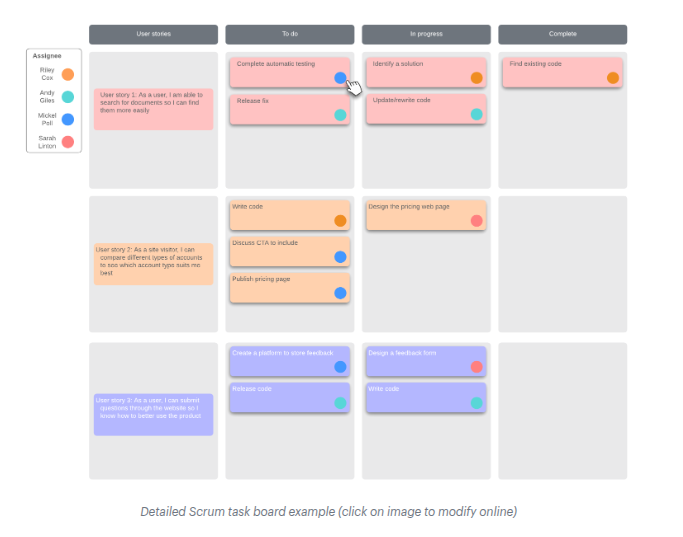
\includegraphics[width=0.8\columnwidth]{image 2.png}
    \caption{The "Scrum for One" methodology, adapted for individual practitioners.}
    \label{fig:scrum_for_one}
\end{figure}

\subsection{The Secure Software Development Lifecycle (SSDLC)}
The SSDLC is a framework for integrating security into every stage of the software development process, from initial design to final deployment. As outlined by Jit [2], the SSDLC promotes a "shift-left" approach to security, where security considerations are addressed early and often. This proactive approach to security is essential for building resilient and trustworthy software systems.

\begin{figure}[h]
    \centering
    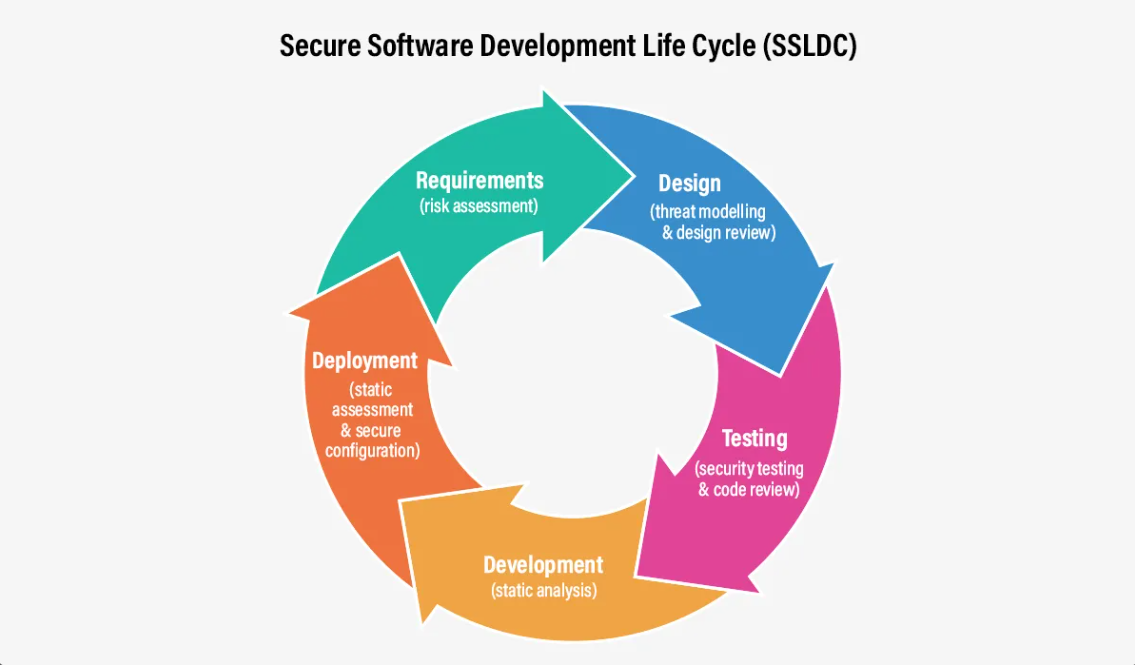
\includegraphics[width=0.8\columnwidth]{image 1.png}
    \caption{The Secure Software Development Lifecycle (SSDLC).}
    \label{fig:ssdlc}
\end{figure}

\subsection{Context Engineering for AIOps}
The effectiveness of any AI system, including AIOps, is highly dependent on the quality of the context it is given. As argued by Schmid [3], "Context Engineering" is the practice of providing AI models with rich, relevant, and timely information to improve their performance. In the context of our proposed framework, this means feeding the AIOps system with data from every stage of the Agile and SSDLC process. This allows the AIOps system to build a comprehensive understanding of the system and provide more accurate and actionable insights.

\begin{figure}[h]
    \centering
    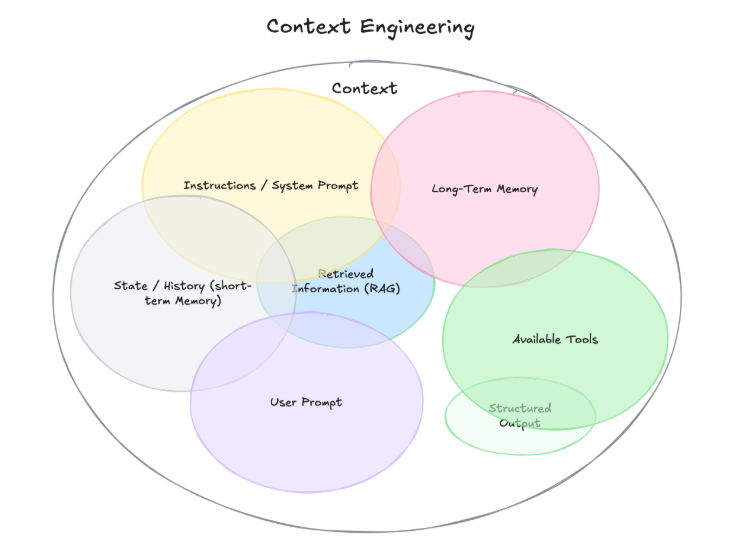
\includegraphics[width=0.8\columnwidth]{image 3.png}
    \caption{Context Engineering for AI Systems.}
    \label{fig:context_engineering}
\end{figure}

\section{The Secure AIOps-driven Agile Framework}
Our proposed framework integrates these three concepts into a cohesive workflow. The framework is cyclical, with each phase feeding into the next, and with AIOps providing a continuous feedback loop.

\begin{enumerate}
    \item \textbf{Sprint Planning (Agile):} The sprint begins with planning, incorporating security requirements (SSDLC) and insights from the AIOps system.
    \item \textbf{Development (Agile + SSDLC):} Developers write code, following secure coding practices and using AI-powered tools for code analysis and completion.
    \item \textbf{Testing (Agile + SSDLC):} The code is tested for both functionality and security vulnerabilities. AIOps can be used to automate test case generation and analysis.
    \item \textbf{Deployment (Agile + AIOps):} The code is deployed, with AIOps monitoring the release for anomalies.
    \item \textbf{Monitoring (AIOps):} The AIOps system continuously monitors the production environment, detecting and responding to incidents.
    \item \textbf{Feedback (AIOps to Agile):} The insights from the AIOps system are fed back into the Agile process, informing the next sprint planning session.
\end{enumerate}

\section{Agent-driven Compliance and Standards}
A key aspect of this framework is the use of machine-readable documentation to enforce standards and compliance. We propose the use of markdown files (e.g., `SUMMARY.md`) within each project directory. These files will underscore the core values and standards of the project. By placing these files in every IDE project, any agent or bot can assess these standards and implement 'guard rails' to ensure compliance. This approach also aids in project reproducibility. By creating `SUMMARY.md` files in each folder that uses the conversation date as a naming convention, we can easily track tangibles and aid others in rebuilding the project from scratch.

\section{Conclusion}
The Secure AIOps-driven Agile Framework provides a roadmap for organizations to build better, more secure software, faster. By integrating Agile, SSDLC, and AIOps, this framework creates a virtuous cycle of continuous improvement, enabling organizations to thrive in the complex and ever-changing world of software development.

\begin{thebibliography}{00}

\bibitem{lucidchart2025}
“Scrum for one: A tutorial on adapting Agile Scrum methodology for individuals,” Lucidchart, Apr. 12, 2025. [Online]. Available: \url{https://www.lucidchart.com/blog/scrum-for-one}

\bibitem{jit2024}
A. Beck and J. Team, “What the Heck is SSDLC (Secure Software Development Lifecycle), and why should devs care?,” Jit, Sep. 17, 2024. [Online]. Available: \url{https://www.jit.io/resources/devsecops/ssdlc-secure-software-development-lifecycle}

\bibitem{schmid2025}
P. Schmid, “The New Skill in AI is Not Prompting, It’s Context Engineering,” The New Skill in AI is Not Prompting, It’s Context Engineering, Jun. 30, 2025. [Online]. Available: \url{https://www.philschmid.de/context-engineering}

\end{thebibliography}

\end{document}
